\section{The Screen Editor}
\label{sec:screen-editor}

When you switch on your MEGA65 or reset it, the following screen will appear:

\begin{center}
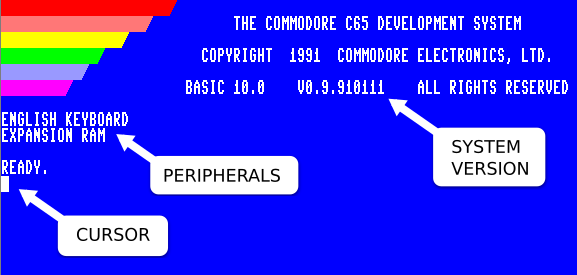
\includegraphics[width={10cm}]{images/introduction-screen/layout.png}
\end{center}

The colour bars in the top left-hand side of the screen can be used
as a guide to help calibrate the colours of your display.
The screen also displays the name of the system,
the copyright notice, and the ROM version.
The displayed date and time are taken from the internal RTC
(Real-Time Clock), which can be set in the Configure Menu.

Finally, you will see the \screentext{READY} prompt and the flashing cursor.

You can begin typing keys on the keyboard and the characters will be
printed at the cursor position. The cursor itself will advance after
each key press.

You can also produce reverse text or colour bars by holding down \specialkey{CTRL} and pressing \megakey{9}, or \megakey{R}. This enters reverse text mode. When this is enabled, you can press and hold the \megakey{Space} bar. While doing so, a white bar will be drawn across the screen.
\index{Keyboard!CTRL}
You can even change the current colour by holding \specialkey{CTRL} down and pressing a number key (from \megakey{1} to \megakey{8}). For example, if you press and hold \specialkey{CTRL} down and press \megakey{1}, the colour will change to black. Now, when you hold down the \megakey{Space} bar, a black bar will be drawn. If you continue to change the colour and press the \megakey{Space} bar, you will get an effect similar to the image below:


\begin{center}
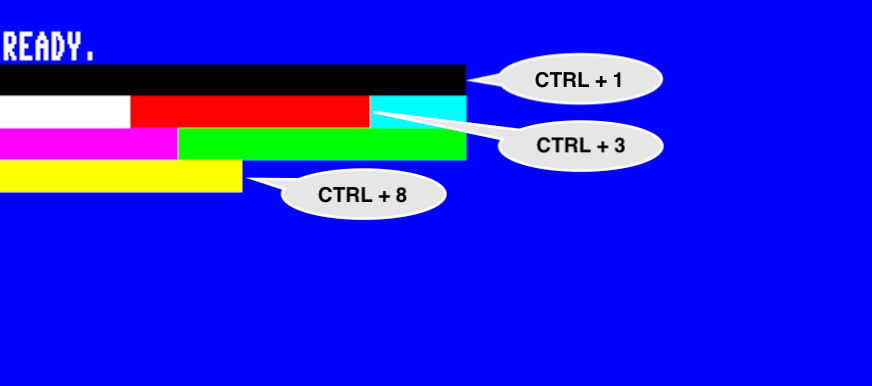
\includegraphics[width={10cm}]{images/introduction-screen/colour-bars.png}
\end{center}


\index{Keyboard!MEGA Key}
You can disable reverse text mode by holding \specialkey{CTRL} and pressing \megakey{0}.

By pressing any key, characters will be printed to the screen in the chosen colour.

A further eight colours can be selected by holding down \megasymbolkey and pressing a key from \megakey{1} to \megakey{8}.
The colour that is printed at the bottom row on the front of the number key will be used. For example, if you held
\megasymbolkey down while pressing \megakey{4}, dark gray will be used. For even more colours, see \bookvref{appendix:escape-colours}.

\needspace{4cm}
You can create fun pictures just by using these colours and letters.  Here's an example of what a year four student drew:

\begin{center}
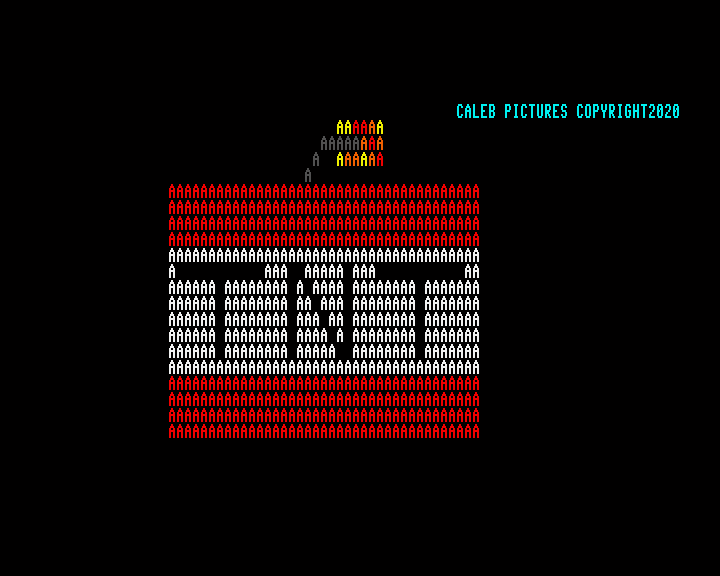
\includegraphics[width={6cm}]{images/caleb-PETSCII-TNT-final}
\end{center}

What will you draw?

\needspace{2cm}
\textbf{Functions}

Functions using \specialkey{CTRL} are called \textbf{Control Codes}.
Functions using \megasymbolkey are called \textbf{Mega Codes}. There are also functions that are called by using \specialkey{SHIFT}, which
are called \textbf{Shifted Codes}.

Lastly, \specialkey{ESC} enables the use of \textbf{Escape Sequences}.

You can read about all of these functions in detail in \bookvref{appendix:controlcodes}, but some are shown in this section.


\needspace{2cm}
\textbf{ESC Sequences}
\index{Keyboard!Escape Sequences}
Escape sequences are performed a little differently than a Control function or a Shift function. Instead of holding the modifier key down, an Escape sequence is performed by pressing \specialkey{ESC} and releasing it, followed by pressing the desired key code.

For example: to switch between 40/80 column mode, press and release \specialkey{ESC}, then press \megakey{X}.

There are more modes available. You can create flashing text by holding \specialkey{CTRL} down and pressing \megakey{O}. Any characters you type in will flash. Turn flash mode off by pressing \specialkey{ESC},  then \megakey{O}.



\section{Editor Functionality}


The MEGA65 screen can allow you to do advanced tabbing, and quickly move around the screen in many ways to help you to be more productive.

For example, press \specialkey{CLR HOME} to go to the home position on the screen. Hold \specialkey{CTRL} down and press \megakey{W} several times. This is the \textbf{Word Advance function}, which jumps your cursor to the next word, or printable character.

You can set custom tab positions on the screen for your convenience. Press \specialkey{CLR HOME} and then \megakey{$\rightarrow$} to the fourth column. Hold down \specialkey{CTRL} and press \megakey{X} to set a tab. Move another 16 positions to the right again, and press \specialkey{CTRL} and \megakey{X} again to set a second tab.

Press \specialkey{CLR HOME} to go back to the home position. Hold \specialkey{CTRL} down and press \megakey{I}. This is the \textbf{Forward Tab function}. Your cursor will tab to the fourth position. Press \specialkey{CTRL} and \megakey{I} again. Your cursor will move to position 8. Why do you ask? By default, every 8th position is already set as a tabbed position. So the 4th and 20th positions have been added to the existing tab positions. You can continue to press \specialkey{CTRL} and \megakey{I} to advance to the 16th and 20th positions.

To find the complete set of Control codes, see \bookvref{appendix:controlcodes}.

\textbf{Creating a Window}
\index{Keyboard!Escape Sequences}

You can set a window on the MEGA65 working screen. Move your cursor to the beginning of the "BASIC 65" text. Press \specialkey{ESC}, then press \megakey{T}. Move the cursor 10 lines down and 15 to the right.

Press \specialkey{ESC}, then \megakey{B}. Anything you type will be contained within this window.

For example, if you were to type \screentext{LIST} to list out a program, the listing will be confined to the window region you have specified:

\begin{center}
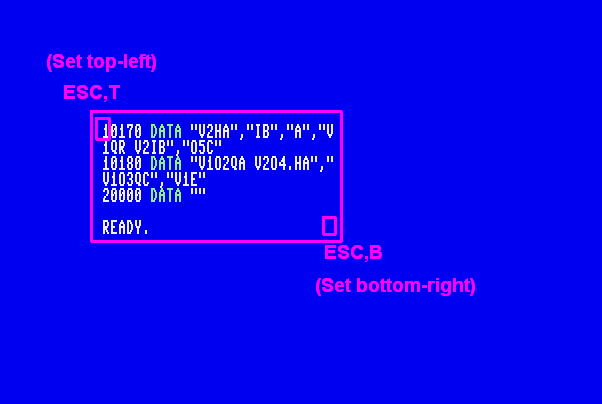
\includegraphics[width={7cm}]{images/set-window.png}
\end{center}

To escape from the window back to the full screen, press \specialkey{CLR HOME} twice.


\textbf{Extras}

Below are some extra, useful things you can do whilst in the screen editor:

  To enter the \textbf{Freeze Menu}, long press on \widekey{RESTORE}, then press \megakey{J} to switch joystick ports without 
having to physically swap the joystick to the other port. You can read more about the Freeze Menu, and what else it can do
on page \pageref{sec:freezer}.

  To enter \textbf{Fast mode} (40.5MHz), either type \screentext{FAST} or \screentext{POKE 0,65} or enter the Freeze Menu and switch the CPU frequency with \megakey{F}.

  Return back to \textbf{Slow mode} (1MHz) by either typing \screentext{FAST 1} or \screentext{POKE 0,64} or enter the Freeze Menu and switch the CPU frequency with \megakey{F}.

  \megasymbolkey + \specialkey{SHIFT} switches between uppercase and lowercase text for the entire display.
